\documentclass[11pt,a4paper]{article}

\usepackage{amsmath,amssymb,amsfonts}
\usepackage[margin=2.5cm]{geometry}
\usepackage{bm}
\usepackage{hyperref}
\usepackage{booktabs}
\usepackage{tikz}
\usetikzlibrary{arrows.meta,positioning,shapes.geometric}

\newcommand{\htlm}{\tilde{h}_{\ell m}}
\newcommand{\Atlm}{\tilde{A}_{\ell m}}
\newcommand{\Philm}{\Phi_{\ell m}}
\newcommand{\Ylm}{{}^{-2}Y_{\ell m}}
\newcommand{\veclambda}{\bm{\lambda}}
\newcommand{\vecchi}{\vec{\chi}}
\newcommand{\Mf}{\mathcal{F}}

\title{Frequency-Domain Waveform Emulation for Gravitational Waves}
\author{Jim Emulators Project}
\date{December 2025}

\begin{document}
\maketitle

\begin{abstract}
We present a framework for neural network emulation of gravitational waveforms in the frequency domain, the natural setting for matched-filter data analysis. The frequency domain offers significant simplifications: extrinsic parameters enter analytically, the mass-scaled frequency $Mf$ provides a universal domain variable, and non-precessing waveforms reduce to smooth amplitude and phase functions without coprecessing frame complications. We detail representation choices, symmetries, and architectural options for neural network emulation, with particular attention to the aligned-spin higher-mode case relevant for IMRPhenomXHM.
\end{abstract}

\tableofcontents
\newpage

%%%%%%%%%%%%%%%%%%%%%%%%%%%%%%%%%%%%%%%%%%%%%%%%%%%%%%%%%%%%%%%%%%%%%%%%%%%%%%%
\section{Introduction}
%%%%%%%%%%%%%%%%%%%%%%%%%%%%%%%%%%%%%%%%%%%%%%%%%%%%%%%%%%%%%%%%%%%%%%%%%%%%%%%

Gravitational wave data analysis operates primarily in the frequency domain. The fundamental detection statistic---the matched filter---is computed as a frequency-domain inner product, and detector noise is characterised by its power spectral density $S_n(f)$. Frequency-domain waveform models (IMRPhenomX, IMRPhenomT, etc.) are the workhorses of LIGO-Virgo-KAGRA parameter estimation.

This document presents a framework for neural network emulation directly in the frequency domain. Compared to time-domain emulation, the frequency domain offers several advantages:

\begin{itemize}
    \item \textbf{Mass scaling}: Waveforms depend on the dimensionless product $Mf$, not mass and frequency separately. This dramatically simplifies the parameter space.
    \item \textbf{Analytic extrinsic dependence}: Distance, coalescence time, and reference phase enter as simple multiplicative factors, eliminating them from the network's learning task.
    \item \textbf{No coprecessing dynamics}: For non-precessing systems, there are no time-evolving Euler angles---just smooth amplitude and phase functions.
    \item \textbf{Direct integration with data analysis}: Emulated waveforms can be used directly in likelihood evaluations without Fourier transformation.
\end{itemize}

For precessing systems, the frequency domain is less natural---precession dynamics are inherently time-domain phenomena that are approximated in frequency-domain models via the ``twisting-up'' procedure. We discuss this and its implications in \S\ref{sec:precession}.

The primary target of this document is emulation of the IMRPhenomXHM family: non-precessing (aligned-spin) waveforms with higher harmonics, computed in the frequency domain.

%%%%%%%%%%%%%%%%%%%%%%%%%%%%%%%%%%%%%%%%%%%%%%%%%%%%%%%%%%%%%%%%%%%%%%%%%%%%%%%
\section{Conventions}
\label{sec:conventions}
%%%%%%%%%%%%%%%%%%%%%%%%%%%%%%%%%%%%%%%%%%%%%%%%%%%%%%%%%%%%%%%%%%%%%%%%%%%%%%%

\paragraph{Complex strain.} The gravitational wave strain is
\begin{equation}
    h \equiv h_+ - i h_\times
    \label{eq:strain_def}
\end{equation}
and its Fourier transform is
\begin{equation}
    \tilde{h}(f) = \int_{-\infty}^{\infty} h(t) \, e^{-2\pi i f t} \, dt
\end{equation}
We work with positive frequencies $f > 0$ throughout; negative frequencies are related by conjugate symmetry of the real time-domain signal.

\paragraph{Geometric units.} We use units with $G = c = 1$, so mass has dimensions of time (or length). The total mass $M = m_1 + m_2$ sets the characteristic timescale. Physical quantities are recovered via:
\begin{align}
    M_{\text{phys}} &= M \times \frac{c^3}{G} = M \times 2.03 \times 10^5 \, M_\odot^{-1} \, \text{s} \\
    f_{\text{phys}} &= \frac{f}{M} \times \frac{c^3}{G M_\odot} = \frac{f}{M/M_\odot} \times 2.03 \times 10^5 \, \text{Hz}
\end{align}

\paragraph{Dimensionless frequency.} The key insight for emulation is that gravitational waveforms depend on the \emph{dimensionless} combination
\begin{equation}
    \boxed{\Mf \equiv M f}
    \label{eq:Mf_def}
\end{equation}
rather than $M$ and $f$ separately. This follows from the scale-invariance of general relativity: there is no intrinsic mass scale in vacuum GR. All time/frequency scales are set by the total mass $M$.

\paragraph{Geometric frequency range.} In geometric units, typical LIGO sources span:
\begin{itemize}
    \item Inspiral onset: $\Mf \sim 10^{-4}$ to $10^{-3}$
    \item Merger: $\Mf \sim 0.01$ to $0.02$
    \item Ringdown: $\Mf \sim 0.05$ to $0.1$
\end{itemize}
A single emulator covering $\Mf \in [10^{-4}, 0.3]$ handles all masses from $1 M_\odot$ to $1000 M_\odot$ across the full LIGO band.

\paragraph{Spin-weighted spherical harmonics.} We use the standard convention for $\Ylm(\iota, \varphi_0)$ consistent with LALSuite and \cite{boyle2011}. Under rotation, modes mix according to the Wigner D-matrices.

\paragraph{Reference frequency.} Waveforms are typically specified at a reference frequency $f_{\rm ref}$ where the orbital phase $\phi_{\rm ref}$ is defined. In terms of $\Mf$, this becomes $\Mf_{\rm ref} = M f_{\rm ref}$.

%%%%%%%%%%%%%%%%%%%%%%%%%%%%%%%%%%%%%%%%%%%%%%%%%%%%%%%%%%%%%%%%%%%%%%%%%%%%%%%
\section{Frequency-Domain Decomposition}
%%%%%%%%%%%%%%%%%%%%%%%%%%%%%%%%%%%%%%%%%%%%%%%%%%%%%%%%%%%%%%%%%%%%%%%%%%%%%%%

\subsection{Spherical Harmonic Expansion}

The frequency-domain strain observed at inclination $\iota$ and reference azimuth $\varphi_0$ is:
\begin{equation}
    \boxed{
    \tilde{h}(f; \veclambda; \iota, \varphi_0) = \sum_{\ell=2}^{\ell_{\max}} \sum_{m=-\ell}^{+\ell} \htlm(f; \veclambda) \, \Ylm(\iota, \varphi_0)
    }
    \label{eq:spherical_harmonic}
\end{equation}
This is identical in form to the time-domain expansion---the Fourier transform is linear, so it commutes with the spherical harmonic sum.

\subsection{Intrinsic vs Extrinsic Parameters}
\label{sec:intrinsic_extrinsic}

A crucial advantage of the frequency domain is that extrinsic parameters enter in simple, analytic ways.

\paragraph{Intrinsic parameters $\veclambda$:} These affect the \emph{shape} of the waveform in $\Mf$ space:
\begin{equation}
    \veclambda = \{\eta, \, \chi_{1z}, \, \chi_{2z}\} \quad \text{(aligned-spin)}
    \label{eq:intrinsic_aligned}
\end{equation}
or more generally:
\begin{equation}
    \veclambda = \{\eta, \, \chi_{1x}, \chi_{1y}, \chi_{1z}, \, \chi_{2x}, \chi_{2y}, \chi_{2z}\} \quad \text{(precessing)}
    \label{eq:intrinsic_precessing}
\end{equation}
where $\eta = m_1 m_2 / (m_1 + m_2)^2$ is the symmetric mass ratio.

\textbf{Note}: The total mass $M$ is \emph{not} an intrinsic parameter for the emulator. The network learns functions of $\Mf$; the mass enters only when converting to physical frequency.

\paragraph{Extrinsic parameters:} Each enters as a simple multiplicative or phase factor:

\begin{enumerate}
    \item \textbf{Total mass $M$}: Converts $\Mf \to f$ and provides the amplitude prefactor. See \S\ref{sec:mass_scaling}.

    \item \textbf{Luminosity distance $D_L$}: Scales amplitude as $\tilde{h} \propto 1/D_L$.

    \item \textbf{Inclination $\iota$ and azimuth $\varphi_0$}: Enter only through $\Ylm(\iota, \varphi_0)$ in \eqref{eq:spherical_harmonic}.

    \item \textbf{Coalescence time $t_c$}: Shifts phase linearly in frequency:
    \begin{equation}
        \htlm(f; t_c) = \htlm(f; t_c = 0) \times e^{-2\pi i f t_c}
        \label{eq:tc_shift}
    \end{equation}

    \item \textbf{Coalescence phase $\phi_c$}: Rotates mode phases:
    \begin{equation}
        \htlm(f; \phi_c) = \htlm(f; \phi_c = 0) \times e^{-i m \phi_c}
        \label{eq:phic_shift}
    \end{equation}

    \item \textbf{Polarisation angle $\psi$}: Mixes $h_+$ and $h_\times$ at the detector (not part of waveform generation).
\end{enumerate}

\paragraph{Implication for emulation.} The neural network learns only the \emph{intrinsic mode shapes}:
\begin{equation}
    \text{NN}: \quad (\Mf, \veclambda) \mapsto \htlm(\Mf; \veclambda)
\end{equation}
All extrinsic parameters are applied analytically at inference time. This reduces the effective parameter space from $\sim 15$ dimensions (full parameter estimation) to 3--7 dimensions (intrinsic only).

\subsection{The Mass Scaling}
\label{sec:mass_scaling}

The dependence on total mass deserves careful treatment. For a waveform at physical frequency $f_{\rm phys}$:
\begin{equation}
    \tilde{h}_{\ell m}(f_{\rm phys}) = \frac{G M}{c^2 D_L} \times \frac{G M}{c^3} \times H_{\ell m}(\Mf; \veclambda)
    \label{eq:mass_scaling}
\end{equation}
where $H_{\ell m}$ is a dimensionless shape function that depends only on $\Mf = G M f_{\rm phys} / c^3$ and intrinsic parameters.

The first factor $GM/c^2 D_L$ is the strain amplitude scale (Schwarzschild radius over distance). The second factor $GM/c^3$ gives the Fourier-transform dimensions (time). Together:
\begin{equation}
    \tilde{h}_{\ell m}(f_{\rm phys}) \propto \frac{M^2}{D_L} \times H_{\ell m}(\Mf; \veclambda)
\end{equation}

\textbf{For emulation}: The network learns $H_{\ell m}(\Mf; \veclambda)$. At inference:
\begin{enumerate}
    \item Given physical parameters $(M, D_L, f_{\rm phys})$, compute $\Mf = M f_{\rm phys}$
    \item Evaluate $H_{\ell m}(\Mf; \veclambda)$ from network
    \item Apply prefactors: $\tilde{h}_{\ell m} = (M^2 / D_L) \times H_{\ell m}$
\end{enumerate}

\subsection{Amplitude--Phase Representation}

Each mode is decomposed into amplitude and phase:
\begin{equation}
    \boxed{
    \htlm(f; \veclambda) = \Atlm(f; \veclambda) \, e^{i \Philm(f; \veclambda)}
    }
    \label{eq:amp_phase}
\end{equation}
where $\Atlm(f) \geq 0$ is the (real, positive) amplitude and $\Philm(f)$ is the (real) phase.

\paragraph{Amplitude characteristics.}
\begin{itemize}
    \item Dynamic range: $\sim 5$ orders of magnitude from low frequency to ringdown
    \item Power-law behaviour in inspiral: $\Atlm \propto f^{-7/6}$ for dominant mode
    \item Peak near merger frequency $\Mf \sim 0.02$
    \item Exponential decay in ringdown
\end{itemize}

\paragraph{Phase characteristics.}
\begin{itemize}
    \item Accumulates $\sim 100$--$200$ radians over typical observation band
    \item Dominated by chirp: $\Philm \propto f^{-5/3}$ at low frequency (Newtonian)
    \item Must be continuous (unwrapped) for learning
    \item Mode phases related: $\Phi_{\ell m} \approx m \times \Phi_{22}/2$ to leading order
\end{itemize}

\paragraph{Practical note.} The amplitude varies over many orders of magnitude while the phase varies over hundreds of radians. These disparate scales suggest different representations (see \S\ref{sec:representation}).

%%%%%%%%%%%%%%%%%%%%%%%%%%%%%%%%%%%%%%%%%%%%%%%%%%%%%%%%%%%%%%%%%%%%%%%%%%%%%%%
\section{Symmetries and Constraints}
\label{sec:symmetries}
%%%%%%%%%%%%%%%%%%%%%%%%%%%%%%%%%%%%%%%%%%%%%%%%%%%%%%%%%%%%%%%%%%%%%%%%%%%%%%%

\subsection{Reality Condition}

The time-domain strain is real: $h(t) = h^*(t)$. In the frequency domain, this implies:
\begin{equation}
    \tilde{h}(-f) = \tilde{h}^*(f)
\end{equation}
We need only model positive frequencies $f > 0$.

\subsection{Conjugate Mode Symmetry (Non-Precessing)}
\label{sec:conjugate_symmetry}

For non-precessing systems with \emph{aligned} spins, the waveform has a reflection symmetry about the orbital plane. This implies:
\begin{equation}
    \boxed{
    \htlm[h_{\ell,-m}](f) = (-1)^\ell \, \htlm^*(f)
    }
    \label{eq:conjugate_symmetry}
\end{equation}

\textbf{Implication for emulation}: We only need to model modes with $m > 0$. The $m < 0$ modes are obtained by conjugation:
\begin{align}
    \tilde{A}_{\ell,-m}(f) &= \Atlm(f) \\
    \Phi_{\ell,-m}(f) &= -\Philm(f) + \ell \pi
\end{align}

For IMRPhenomXHM, the relevant positive-$m$ modes are: $(2,2)$, $(2,1)$, $(3,3)$, $(3,2)$, $(4,4)$.

\subsection{Mode Hierarchy}

Not all modes contribute equally:

\begin{table}[h]
\centering
\begin{tabular}{lcc}
\toprule
\textbf{Mode} & \textbf{Relative Amplitude} & \textbf{Peak Frequency} \\
\midrule
$(2,2)$ & 1 (reference) & $\Mf \approx 0.02$ \\
$(2,1)$ & $\sim 0.1$--$0.3$ & $\Mf \approx 0.01$ \\
$(3,3)$ & $\sim 0.05$--$0.3$ & $\Mf \approx 0.03$ \\
$(3,2)$ & $\sim 0.01$--$0.1$ & $\Mf \approx 0.02$ \\
$(4,4)$ & $\sim 0.01$--$0.1$ & $\Mf \approx 0.04$ \\
\bottomrule
\end{tabular}
\caption{Approximate mode amplitudes relative to $(2,2)$, depending on mass ratio and spins.}
\label{tab:modes}
\end{table}

Higher modes become more important for:
\begin{itemize}
    \item Unequal masses ($q \neq 1$)
    \item Edge-on inclinations ($\iota \approx \pi/2$)
    \item Higher total masses (where fewer inspiral cycles are in band)
\end{itemize}

\subsection{Phase Conventions and Degeneracies}

Several phase parameters are partially degenerate:
\begin{itemize}
    \item \textbf{Reference phase} $\phi_{\rm ref}$: The phase of the $(2,2)$ mode at reference frequency
    \item \textbf{Coalescence phase} $\phi_c$: The orbital phase at coalescence
    \item \textbf{Azimuthal angle} $\varphi_0$: Viewing angle in orbital plane
\end{itemize}

For data analysis, only certain combinations are measurable. For emulation, we fix a convention:
\begin{equation}
    \Phi_{22}(\Mf_{\rm ref}) = 0
\end{equation}
This removes the phase freedom in training data.

%%%%%%%%%%%%%%%%%%%%%%%%%%%%%%%%%%%%%%%%%%%%%%%%%%%%%%%%%%%%%%%%%%%%%%%%%%%%%%%
\section{Representation Choices for Neural Networks}
\label{sec:representation}
%%%%%%%%%%%%%%%%%%%%%%%%%%%%%%%%%%%%%%%%%%%%%%%%%%%%%%%%%%%%%%%%%%%%%%%%%%%%%%%

\subsection{Amplitude Representation}

The amplitude $\Atlm(\Mf)$ spans $\sim 5$ orders of magnitude. Direct representation is challenging for neural networks. Options:

\paragraph{Option A: Log-amplitude.}
\begin{equation}
    \text{Output}: \quad \log \Atlm(\Mf)
\end{equation}
\textbf{Pros}: Handles dynamic range naturally, errors become relative \\
\textbf{Cons}: Undefined when $\Atlm \to 0$ (mode zeros), log-errors weight low amplitudes heavily

\paragraph{Option B: Normalised amplitude.}
\begin{equation}
    \text{Output}: \quad \frac{\Atlm(\Mf)}{\tilde{A}_{22}^{\rm ref}(\Mf)}
\end{equation}
where $\tilde{A}_{22}^{\rm ref}$ is a reference $(2,2)$ amplitude (e.g., at $\eta = 0.25$, $\chi = 0$).

\textbf{Pros}: Order-unity outputs, physically motivated \\
\textbf{Cons}: Requires reference waveform, extra preprocessing

\paragraph{Option C: Post-Newtonian subtraction.}
\begin{equation}
    \text{Output}: \quad \frac{\Atlm(\Mf)}{\Atlm^{\rm PN}(\Mf)}
\end{equation}
where $\Atlm^{\rm PN}$ is the leading-order post-Newtonian amplitude.

\textbf{Pros}: Network learns only the ``correction'' to known physics \\
\textbf{Cons}: PN diverges at merger, need transition handling

\paragraph{Recommendation}: Log-amplitude (Option A) for its simplicity, with careful handling of mode zeros if they occur in the training data.

\subsection{Phase Representation}

The phase $\Philm(\Mf)$ accumulates hundreds of radians. Options:

\paragraph{Option A: Direct (unwrapped) phase.}
\begin{equation}
    \text{Output}: \quad \Philm(\Mf)
\end{equation}
\textbf{Pros}: Simple, direct \\
\textbf{Cons}: Large dynamic range, errors in radians may be acceptable but scale poorly

\paragraph{Option B: Phase derivative (instantaneous frequency).}
\begin{equation}
    \text{Output}: \quad \frac{d\Philm}{d(\Mf)} = \omega_{\ell m}(\Mf)
\end{equation}
Reconstruct phase by integration: $\Philm(\Mf) = \int^{\Mf} \omega_{\ell m} \, d(\Mf')$

\textbf{Pros}: Bounded output, physical interpretation (GW frequency) \\
\textbf{Cons}: Integration accumulates errors, boundary condition needed

\paragraph{Option C: Residual after PN subtraction.}
\begin{equation}
    \text{Output}: \quad \Philm(\Mf) - \Philm^{\rm PN}(\Mf; \veclambda)
\end{equation}
where $\Philm^{\rm PN}$ is the post-Newtonian phase to high order.

\textbf{Pros}: Network learns small corrections, PN is well-understood \\
\textbf{Cons}: PN coefficients depend on parameters, need to evaluate PN at inference

\paragraph{Option D: TaylorF2 residual.}
\begin{equation}
    \text{Output}: \quad \Philm(\Mf) - \Philm^{\rm TF2}(\Mf; \veclambda)
\end{equation}
where $\Philm^{\rm TF2}$ is the TaylorF2 phase (analytic PN in frequency domain).

\textbf{Pros}: TaylorF2 is fast to evaluate, captures bulk of inspiral phase \\
\textbf{Cons}: Breaks down at merger, need smooth transition

\paragraph{Recommendation}: For initial implementation, direct phase (Option A) with unwrapping. For production accuracy, consider PN residual (Option C/D) to reduce the dynamic range the network must capture.

\subsection{Frequency Grid}
\label{sec:frequency_grid}

The network can operate on:

\paragraph{Fixed grid in $\Mf$.}
Train and evaluate on a fixed set of geometric frequencies $\{\Mf_1, \Mf_2, \ldots, \Mf_N\}$.

\textbf{Grid spacing}: The waveform has features on different scales:
\begin{itemize}
    \item Inspiral: Slowly varying, coarse grid sufficient
    \item Merger: Rapid variation, fine grid needed
    \item Ringdown: Quasi-periodic, moderate grid
\end{itemize}

A log-spaced grid is natural, matching the power-law inspiral behaviour:
\begin{equation}
    \Mf_k = \Mf_{\min} \times \left( \frac{\Mf_{\max}}{\Mf_{\min}} \right)^{k/N}, \quad k = 0, \ldots, N
\end{equation}

\paragraph{Continuous evaluation.}
Instead of a fixed grid, output basis coefficients that allow evaluation at any $\Mf$:
\begin{equation}
    \Atlm(\Mf) = \sum_{k=1}^{K} c^{(A)}_k(\veclambda) \, B_k(\Mf)
\end{equation}
where $B_k(\Mf)$ are basis functions (splines, PCA modes, etc.).

\textbf{Pros}: Arbitrary resolution at inference, interpolation is exact within basis \\
\textbf{Cons}: More complex architecture, basis must be chosen carefully

\paragraph{Recommendation}: For initial implementation, use a fixed log-spaced grid with $\sim 1000$ points. Interpolate for intermediate frequencies if needed.

%%%%%%%%%%%%%%%%%%%%%%%%%%%%%%%%%%%%%%%%%%%%%%%%%%%%%%%%%%%%%%%%%%%%%%%%%%%%%%%
\section{Neural Network Architecture}
\label{sec:architecture}
%%%%%%%%%%%%%%%%%%%%%%%%%%%%%%%%%%%%%%%%%%%%%%%%%%%%%%%%%%%%%%%%%%%%%%%%%%%%%%%

\subsection{Direct Mapping (Per-Frequency)}
\label{sec:arch_direct}

The simplest architecture evaluates each frequency independently:

\begin{center}
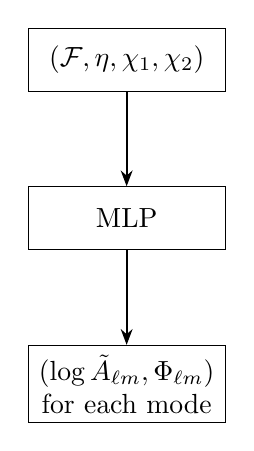
\begin{tikzpicture}[
    node distance=1.2cm,
    box/.style={rectangle, draw, minimum width=2.5cm, minimum height=0.8cm, align=center},
    arrow/.style={-{Stealth[length=2mm]}, thick}
]
    \node[box] (input) {$(\Mf, \eta, \chi_1, \chi_2)$};
    \node[box, below=of input] (nn) {MLP};
    \node[box, below=of nn] (output) {$(\log \Atlm, \Philm)$\\for each mode};

    \draw[arrow] (input) -- (nn);
    \draw[arrow] (nn) -- (output);
\end{tikzpicture}
\end{center}

\textbf{Pros}: Simple, embarrassingly parallel over frequencies \\
\textbf{Cons}: Doesn't exploit correlations across frequency, large network needed

\subsection{PCA + MLP (CosmoPower Architecture)}
\label{sec:arch_pca}

Following CosmoPower \cite{cosmopower}:

\begin{enumerate}
    \item \textbf{Training data}: Generate waveforms on fixed grid for many parameter values
    \item \textbf{PCA}: Compute principal components across training set
    \item \textbf{Network}: MLP maps parameters to PCA coefficients
    \item \textbf{Reconstruction}: Combine PCA modes to get waveform
\end{enumerate}

\begin{center}
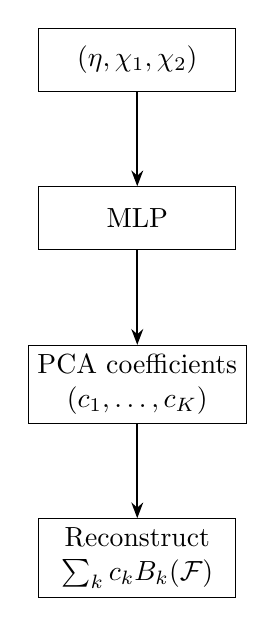
\begin{tikzpicture}[
    node distance=1.2cm,
    box/.style={rectangle, draw, minimum width=2.5cm, minimum height=0.8cm, align=center},
    arrow/.style={-{Stealth[length=2mm]}, thick}
]
    \node[box] (input) {$(\eta, \chi_1, \chi_2)$};
    \node[box, below=of input] (nn) {MLP};
    \node[box, below=of nn] (pca) {PCA coefficients\\$(c_1, \ldots, c_K)$};
    \node[box, below=of pca] (output) {Reconstruct\\$\sum_k c_k B_k(\Mf)$};

    \draw[arrow] (input) -- (nn);
    \draw[arrow] (nn) -- (pca);
    \draw[arrow] (pca) -- (output);
\end{tikzpicture}
\end{center}

\textbf{Pros}: Exploits waveform correlations, compact representation, CosmoPower-validated \\
\textbf{Cons}: Separate PCA for each quantity (amplitude, phase, per mode), fixed frequency grid

\subsection{Mode-Coupled Architecture}
\label{sec:arch_coupled}

Higher modes are correlated with the $(2,2)$ mode (they come from the same binary). A coupled architecture can exploit this:

\begin{center}
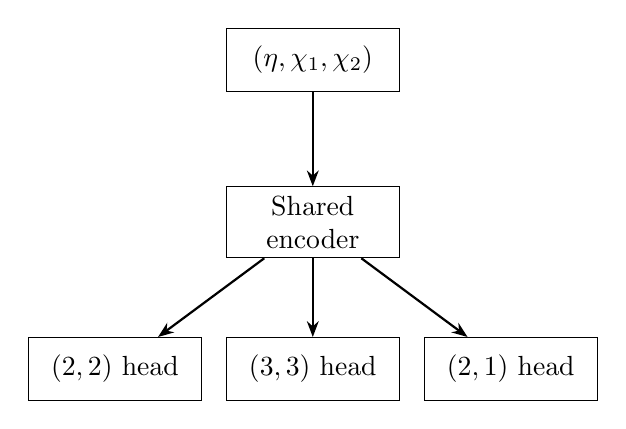
\begin{tikzpicture}[
    node distance=1.2cm,
    box/.style={rectangle, draw, minimum width=2.2cm, minimum height=0.8cm, align=center},
    arrow/.style={-{Stealth[length=2mm]}, thick}
]
    \node[box] (input) {$(\eta, \chi_1, \chi_2)$};
    \node[box, below=of input] (shared) {Shared\\encoder};
    \node[box, below left=1cm and 0.3cm of shared] (h22) {$(2,2)$ head};
    \node[box, below=1cm of shared] (h33) {$(3,3)$ head};
    \node[box, below right=1cm and 0.3cm of shared] (h21) {$(2,1)$ head};

    \draw[arrow] (input) -- (shared);
    \draw[arrow] (shared) -- (h22);
    \draw[arrow] (shared) -- (h33);
    \draw[arrow] (shared) -- (h21);
\end{tikzpicture}
\end{center}

\textbf{Pros}: Shared features, potentially smaller total network \\
\textbf{Cons}: More complex, mode dependencies may not help much

\subsection{Recommended Starting Point}

For initial development, we recommend:

\begin{enumerate}
    \item \textbf{PCA + MLP architecture} (CosmoPower-style)
    \item \textbf{Separate models per mode} initially, unify later if beneficial
    \item \textbf{Log-amplitude} and \textbf{direct phase} outputs
    \item \textbf{Log-spaced grid} in $\Mf$
    \item \textbf{Speculator activation function} $\sigma(x) = x \cdot \text{sigmoid}(x)$ \cite{speculator}
\end{enumerate}

%%%%%%%%%%%%%%%%%%%%%%%%%%%%%%%%%%%%%%%%%%%%%%%%%%%%%%%%%%%%%%%%%%%%%%%%%%%%%%%
\section{The Precessing Case}
\label{sec:precession}
%%%%%%%%%%%%%%%%%%%%%%%%%%%%%%%%%%%%%%%%%%%%%%%%%%%%%%%%%%%%%%%%%%%%%%%%%%%%%%%

For precessing systems, frequency-domain modelling is more complex. The time-domain coprecessing frame decomposition does not have a direct frequency-domain analog because the Euler angles $\alpha(t), \beta(t), \gamma(t)$ are functions of time, not frequency.

\subsection{The Twisting-Up Approximation}

IMRPhenomXPHM and similar models use the ``twisting-up'' approach:

\begin{enumerate}
    \item Compute non-precessing (aligned-spin) modes in frequency domain
    \item Apply frequency-dependent rotation to account for precession
\end{enumerate}

The key approximation is the \textbf{stationary phase assumption}: each frequency component $f$ corresponds to a single time $t(f)$ via the time-frequency relation of the dominant mode. The Euler angles at that time, $\alpha(t(f)), \beta(t(f)), \gamma(t(f))$, are then used to rotate the modes:

\begin{equation}
    \htlm(f) = \sum_{m'=-\ell}^{+\ell} D^\ell_{mm'}\bigl(\alpha(t(f)), \beta(t(f)), \gamma(t(f))\bigr) \, \tilde{h}^{\rm AS}_{\ell m'}(f)
\end{equation}
where $\tilde{h}^{\rm AS}$ are aligned-spin modes.

\subsection{Limitations of Frequency-Domain Precession}

The twisting-up approach has known limitations:
\begin{itemize}
    \item \textbf{Mode mixing}: Power can leak between modes during precession
    \item \textbf{Multiple timescales}: Strong precession violates stationary phase
    \item \textbf{Transitional precession}: Near $L \sim S$, the frame can flip rapidly
\end{itemize}

For highly precessing systems, time-domain modelling (as in the companion document) may be more appropriate.

\subsection{Emulation Strategy for Precessing Waveforms}

Two approaches for emulating precessing frequency-domain waveforms:

\paragraph{Option 1: Emulate the twisted output.}
Treat the full $\htlm(f; \veclambda)$ including precession as the target. The network learns the combined effect of mode evolution and precession.

\textbf{Pros}: Simple, single network \\
\textbf{Cons}: Must learn oscillatory structure from precession, larger network needed

\paragraph{Option 2: Emulate components separately.}
Train separate networks for:
\begin{itemize}
    \item Aligned-spin modes $\tilde{h}^{\rm AS}_{\ell m'}(f)$
    \item Euler angles as functions of frequency $\alpha(f), \beta(f), \gamma(f)$
\end{itemize}
Combine via Wigner rotation at inference.

\textbf{Pros}: Modular, aligned-spin emulator can be reused \\
\textbf{Cons}: Two networks, angle-frequency relation approximate

\paragraph{Recommendation}: For this project, focus on non-precessing (aligned-spin) waveforms first. Precession can be added later following Option 2, building on the aligned-spin emulator.

%%%%%%%%%%%%%%%%%%%%%%%%%%%%%%%%%%%%%%%%%%%%%%%%%%%%%%%%%%%%%%%%%%%%%%%%%%%%%%%
\section{Training and Validation}
\label{sec:training}
%%%%%%%%%%%%%%%%%%%%%%%%%%%%%%%%%%%%%%%%%%%%%%%%%%%%%%%%%%%%%%%%%%%%%%%%%%%%%%%

\subsection{Training Data Generation}

\paragraph{Parameter sampling.}
\begin{itemize}
    \item \textbf{Symmetric mass ratio} $\eta \in [0.05, 0.25]$ (mass ratios $q \in [1, 18]$)
    \item \textbf{Spin components} $\chi_{1z}, \chi_{2z} \in [-0.99, 0.99]$
    \item \textbf{Sampling}: Latin hypercube or Sobol sequence for space-filling
    \item \textbf{Training set size}: $\sim 10^4$--$10^5$ waveforms
\end{itemize}

\paragraph{Waveform generation.}
Use LALSimulation to generate IMRPhenomXHM waveforms:
\begin{verbatim}
from lal import MSUN_SI
import lalsimulation as lalsim

hp, hc = lalsim.SimIMRPhenomXHM(
    m1_SI, m2_SI, S1z, S2z,  # masses and spins
    distance, inclination,   # extrinsic (set to reference)
    phiRef, deltaF, f_min,   # frequency grid
    f_ref, lalParams         # reference and options
)
\end{verbatim}

\paragraph{Data format.}
Store in HDF5:
\begin{itemize}
    \item Frequency grid: $\Mf$ values (common to all waveforms)
    \item Per waveform: parameters $(\eta, \chi_1, \chi_2)$, amplitudes, phases for each mode
    \item Metadata: LAL version, waveform approximant, options used
\end{itemize}

\subsection{Loss Functions}

\paragraph{Mean squared error.}
On log-amplitude and phase:
\begin{equation}
    \mathcal{L}_{\rm MSE} = \sum_{\ell m} \left[ \left\| \log \Atlm^{\rm pred} - \log \Atlm^{\rm true} \right\|^2 + w_\Phi \left\| \Philm^{\rm pred} - \Philm^{\rm true} \right\|^2 \right]
\end{equation}
where $w_\Phi$ balances amplitude and phase contributions.

\paragraph{Complex MSE.}
Directly on the complex waveform:
\begin{equation}
    \mathcal{L}_{\rm complex} = \sum_{\ell m} \left\| \htlm^{\rm pred} - \htlm^{\rm true} \right\|^2
\end{equation}
This automatically balances amplitude and phase.

\subsection{Validation: The Mismatch}
\label{sec:mismatch}

The standard accuracy metric for gravitational waveforms is the \textbf{mismatch}:
\begin{equation}
    \boxed{
    \mathcal{M} = 1 - \max_{t_c, \phi_c} \frac{\langle h_1 | h_2 \rangle}{\sqrt{\langle h_1 | h_1 \rangle \langle h_2 | h_2 \rangle}}
    }
    \label{eq:mismatch}
\end{equation}
where the noise-weighted inner product is:
\begin{equation}
    \langle h_1 | h_2 \rangle = 4 \, \text{Re} \int_{f_{\rm low}}^{f_{\rm high}} \frac{\tilde{h}_1(f) \tilde{h}_2^*(f)}{S_n(f)} \, df
\end{equation}
and $S_n(f)$ is the detector noise power spectral density.

\paragraph{Target accuracy.}
For parameter estimation, mismatches $\lesssim 10^{-3}$ are typically required. This corresponds to:
\begin{itemize}
    \item Amplitude errors: $\lesssim 1\%$ relative
    \item Phase errors: $\lesssim 0.1$ radians
\end{itemize}

\paragraph{Mismatch as loss function.}
The mismatch can be used directly as a loss function, but requires:
\begin{itemize}
    \item Differentiable inner product implementation
    \item Handling of maximisation over $t_c$, $\phi_c$
    \item Choice of reference PSD $S_n(f)$
\end{itemize}

For initial training, MSE is simpler. Mismatch is better suited for validation and fine-tuning.

%%%%%%%%%%%%%%%%%%%%%%%%%%%%%%%%%%%%%%%%%%%%%%%%%%%%%%%%%%%%%%%%%%%%%%%%%%%%%%%
\section{Comparison with Time-Domain Framework}
\label{sec:comparison}
%%%%%%%%%%%%%%%%%%%%%%%%%%%%%%%%%%%%%%%%%%%%%%%%%%%%%%%%%%%%%%%%%%%%%%%%%%%%%%%

\begin{table}[h]
\centering
\begin{tabular}{lcc}
\toprule
\textbf{Aspect} & \textbf{Time Domain} & \textbf{Frequency Domain} \\
\midrule
Natural domain variable & $t/M$ & $Mf$ \\
Coprecessing frame needed & Yes (precessing) & No (approximated) \\
Euler angle dynamics & Learned & Derived from $t(f)$ \\
Extrinsic parameters & Mixed in & Analytic factors \\
Phase accumulation & Implicit & Explicit (many radians) \\
Mode mixing & Via Wigner rotation & Via twisting-up \\
Direct data analysis use & Requires FFT & Yes \\
\midrule
Best for & Precessing, eccentric & Aligned-spin, circular \\
\bottomrule
\end{tabular}
\caption{Comparison of time-domain and frequency-domain emulation frameworks.}
\label{tab:comparison}
\end{table}

The two frameworks are complementary:
\begin{itemize}
    \item \textbf{Frequency domain}: Simpler for non-precessing waveforms, direct use in data analysis, cleaner mass scaling
    \item \textbf{Time domain}: More natural for precession, handles multiple timescales, needed for eccentric systems
\end{itemize}

For this project (IMRPhenomXHM emulation), the frequency domain is the natural choice.

%%%%%%%%%%%%%%%%%%%%%%%%%%%%%%%%%%%%%%%%%%%%%%%%%%%%%%%%%%%%%%%%%%%%%%%%%%%%%%%
\section{Summary}
%%%%%%%%%%%%%%%%%%%%%%%%%%%%%%%%%%%%%%%%%%%%%%%%%%%%%%%%%%%%%%%%%%%%%%%%%%%%%%%

The frequency-domain framework for waveform emulation is:

\begin{align}
    \tilde{h}(f; \veclambda; \iota, \varphi_0) &= \sum_{\ell, m} \htlm(f; \veclambda) \, \Ylm(\iota, \varphi_0) \\[0.5em]
    \htlm(f; \veclambda) &= \Atlm(f; \veclambda) \, e^{i \Philm(f; \veclambda)} \\[0.5em]
    \text{NN}: (\Mf, \veclambda) &\mapsto (\log \Atlm, \Philm) \quad \text{for each mode}
\end{align}

\textbf{Key points}:
\begin{enumerate}
    \item The dimensionless frequency $\Mf = Mf$ is the natural domain variable---total mass is not an intrinsic parameter.
    \item Extrinsic parameters (distance, coalescence time/phase, inclination) enter analytically via simple multiplicative factors.
    \item For non-precessing systems, conjugate symmetry halves the number of modes to emulate.
    \item Log-amplitude and direct phase are suitable output representations for neural networks.
    \item The PCA + MLP architecture (CosmoPower-style) is a proven approach.
    \item Mismatch is the standard validation metric; target $\mathcal{M} < 10^{-3}$.
    \item Precessing waveforms can be added via separate Euler angle emulation (twisting-up), building on the aligned-spin base.
\end{enumerate}

\textbf{Recommended starting point}: Emulate IMRPhenomXHM modes $(2,2)$, $(2,1)$, $(3,3)$, $(3,2)$, $(4,4)$ for aligned-spin parameter space $(\eta, \chi_{1z}, \chi_{2z})$ using PCA + MLP architecture with log-amplitude and unwrapped phase outputs.

%%%%%%%%%%%%%%%%%%%%%%%%%%%%%%%%%%%%%%%%%%%%%%%%%%%%%%%%%%%%%%%%%%%%%%%%%%%%%%%
\begin{thebibliography}{99}

\bibitem{boyle2011}
M.~Boyle, R.~Owen, H.~P.~Pfeiffer,
``A geometric approach to the precession of compact binaries,''
Phys.\ Rev.\ D \textbf{84}, 124011 (2011), arXiv:1110.2965.

\bibitem{cosmopower}
A.~Spurio Mancini, D.~Piras, J.~Alsing, B.~Joachimi, M.~P.~Hobson,
``CosmoPower: emulating cosmological power spectra for accelerated Bayesian inference from next-generation surveys,''
Mon.\ Not.\ Roy.\ Astron.\ Soc.\ \textbf{511}, 1771 (2022), arXiv:2106.03846.

\bibitem{speculator}
J.~Alsing, B.~Wandelt, S.~Feeney,
``Speculator: Emulating stellar population synthesis for fast and accurate galaxy spectra and photometry,''
Astrophys.\ J.\ Suppl.\ \textbf{249}, 5 (2020), arXiv:1911.11778.

\bibitem{phenomxhm}
C.~Garc\'ia-Quir\'os, M.~Colleoni, S.~Husa, H.~Estell\'es, G.~Pratten, A.~Ramos-Buades, M.~Mateu-Lucena, R.~Jaume,
``IMRPhenomXHM: A multi-mode frequency-domain model for the gravitational wave signal from non-precessing black-hole binaries,''
Phys.\ Rev.\ D \textbf{102}, 064002 (2020), arXiv:2001.10914.

\bibitem{phenomxphm}
G.~Pratten et al.,
``Computationally efficient models for the dominant and subdominant harmonic modes of precessing binary black holes,''
Phys.\ Rev.\ D \textbf{103}, 104056 (2021), arXiv:2004.06503.

\end{thebibliography}

\end{document}
